\documentclass[aspectratio=169]{beamer}

% =====================================================================
% DECK 09 -- the engraving aesthetic, content presented PROFESSIONALLY.
% Warm paper, EB Garamond, pen-and-ink accents; but real structure:
% titled slides, bullet points, data tables, clear takeaways. The
% illustrations are small supporting emblems, not the whole slide.
% =====================================================================

\usepackage[T1]{fontenc}
\usepackage{ebgaramond}
\renewcommand{\familydefault}{\rmdefault}
\usepackage{tikz}
\usepackage{booktabs}
\usepackage{array}
\usetikzlibrary{decorations.pathmorphing, calc, arrows.meta, shapes.misc, positioning}

\usetheme{default}
\usefonttheme{professionalfonts}
\setbeamertemplate{navigation symbols}{}

\definecolor{paper}{HTML}{FAF7EF}
\definecolor{ink}{HTML}{211E18}
\definecolor{inkl}{HTML}{6B6557}
\definecolor{accent}{HTML}{8A3324}
\definecolor{wsky}{HTML}{8FB0C9}
\definecolor{wwater}{HTML}{6E97B5}
\definecolor{wgreen}{HTML}{7E9347}
\definecolor{wamber}{HTML}{DBA23E}
\definecolor{wochre}{HTML}{B5824A}
\definecolor{wred}{HTML}{C24B43}
\definecolor{wviolet}{HTML}{8A6BA8}
\definecolor{wteal}{HTML}{3E9C8F}
\definecolor{wgold}{HTML}{CCA63E}

\setbeamercolor{background canvas}{bg=paper}
\setbeamercolor{normal text}{fg=ink}
\setbeamercolor{frametitle}{fg=ink}
\setbeamercolor{itemize item}{fg=inkl}
\setbeamercolor{itemize subitem}{fg=inkl}
\setbeamercolor{block title}{fg=paper, bg=ink}
\setbeamercolor{block body}{fg=ink, bg=ink!6}
\setbeamerfont{frametitle}{size=\Large}
\setbeamerfont{block title}{series=\scshape}

\setbeamertemplate{itemize item}{\small\textendash}
\setbeamertemplate{itemize subitem}{\textperiodcentered}
\setbeamertemplate{itemize subsubitem}{\textperiodcentered}
\setlength{\leftmargini}{1.4em}
\renewcommand{\arraystretch}{1.18}

% engraved-plate frame title: small caps + thin rule
\setbeamertemplate{frametitle}{%
  \vskip0.5em
  \leavevmode\hbox{\hskip0.2em{\scshape\Large\insertframetitle}}%
  \vskip0.12em
  \hbox{\hskip0.2em{\color{inkl}\rule{0.955\paperwidth}{0.4pt}}}%
  \vskip0.2em}

\setbeamertemplate{footline}{%
  \vskip2pt
  \hbox to\paperwidth{\hskip0.45cm{\color{inkl}\scriptsize\scshape Rotor in Rust}%
     \hfill{\color{inkl}\scriptsize\insertframenumber\,/\,\inserttotalframenumber}\hskip0.45cm}%
  \vskip3pt}

\newcommand{\key}[1]{{\color{accent}\textbf{#1}}}

% ---- small engraved emblems -----------------------------------------------
\tikzset{el/.style={line cap=round, line join=round}}

\newcommand{\engMountains}{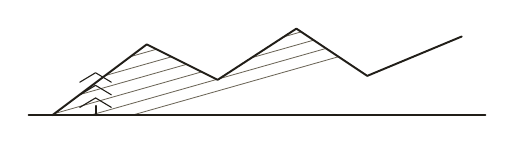
\begin{tikzpicture}[el]
  \begin{scope}\clip (-2.6,0)--(-1.4,0.9)--(-0.5,0.45)--(0.5,1.1)--(1.4,0.5)--(2.6,1.0)--(2.6,0)--cycle;
     \foreach \hy in {-0.4,-0.25,...,1.1}{\draw[inkl,line width=0.3pt] (-3,\hy)--(3,\hy+1.7);}\end{scope}
  \draw[ink,line width=0.7pt] (-2.6,0)--(-1.4,0.9)--(-0.5,0.45)--(0.5,1.1)--(1.4,0.5)--(2.6,1.0);
  \draw[ink,line width=0.7pt] (-2.9,0)--(2.9,0);
  \draw[ink,line width=0.7pt] (-2.05,0)--(-2.05,0.12);
  \foreach \ty in {0.10,0.26,0.42}{\draw[ink,line width=0.4pt] (-2.05,\ty+0.12)--(-2.25,\ty) (-2.05,\ty+0.12)--(-1.85,\ty);}
\end{tikzpicture}}

\newcommand{\engSun}{
\begin{tikzpicture}[el]
  \begin{scope}\clip (0,0) circle (0.72);
    \fill[wamber!35] (-1,-1) rectangle (1,1);
    \foreach \hy in {-0.6,-0.45,...,0.6}{\draw[inkl, line width=0.3pt] (-1,\hy)--(1,\hy+0.85);}\end{scope}
  \draw[ink, line width=0.9pt] (0,0) circle (0.72);
  \foreach \a in {0,22.5,...,337.5}{\draw[ink, line width=0.35pt] (\a:0.88)--(\a:{1.08+0.12*abs(sin(\a*2))});}
\end{tikzpicture}}

\newcommand{\engGear}{
\begin{tikzpicture}[el]
  \foreach \i in {0,...,23}{\pgfmathsetmacro{\a}{\i*15}
     \fill[ink] (\a-3.5:0.95) -- (\a-3.5:1.12) -- (\a+3.5:1.12) -- (\a+3.5:0.95) -- cycle;}
  \begin{scope}\clip (0,0) circle (0.95);
     \fill[wgold!35] (-1,-1) rectangle (1,1);
     \foreach \hy in {-0.9,-0.74,...,0.9}{\draw[inkl, line width=0.3pt] (-1.2,\hy)--(1.2,\hy+0.6);}\end{scope}
  \draw[ink, line width=0.9pt] (0,0) circle (0.95);
  \fill[paper] (0,0) circle (0.42);\draw[ink, line width=0.7pt] (0,0) circle (0.42);
\end{tikzpicture}}

\newcommand{\engChest}{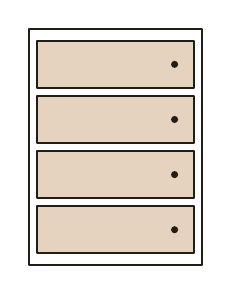
\begin{tikzpicture}[el]
  \draw[ink, line width=0.9pt] (-1.1,-1.5) rectangle (1.1,1.5);
  \foreach \y in {1.05,0.35,-0.35,-1.05}{
     \begin{scope}\clip (-1.0,\y-0.3) rectangle (1.0,\y+0.3);\fill[wochre!35] (-1.2,\y-0.4) rectangle (1.2,\y+0.4);\end{scope}
     \draw[ink, line width=0.6pt] (-1.0,\y-0.3) rectangle (1.0,\y+0.3);
     \fill[ink] (0.75,\y) circle (0.045);}
\end{tikzpicture}}

\newcommand{\engHourglass}{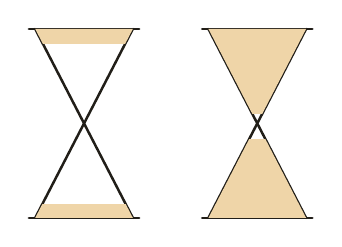
\begin{tikzpicture}[el]
  \foreach \x/\topf in {0/0.85, 2.2/0.1}{
     \draw[ink, line width=0.9pt] (\x-0.7,1.2)--(\x+0.7,1.2) (\x-0.7,-1.2)--(\x+0.7,-1.2);
     \draw[ink, line width=0.9pt] (\x-0.62,1.2)--(\x,0)--(\x-0.62,-1.2);
     \draw[ink, line width=0.9pt] (\x+0.62,1.2)--(\x,0)--(\x+0.62,-1.2);
     \begin{scope}\clip (\x-0.62,1.2)--(\x,0)--(\x+0.62,1.2)--cycle;
        \clip (\x-0.7,{0+\topf*1.2}) rectangle (\x+0.7,1.2);\fill[wamber!45] (\x-1,0) rectangle (\x+1,1.3);\end{scope}
     \begin{scope}\clip (\x-0.62,-1.2)--(\x,0)--(\x+0.62,-1.2)--cycle;
        \clip (\x-0.7,-1.2) rectangle (\x+0.7,{-1.2+(1-\topf)*1.1});\fill[wamber!45] (\x-1,-1.3) rectangle (\x+1,0);\end{scope}}
\end{tikzpicture}}

\newcommand{\engBalance}{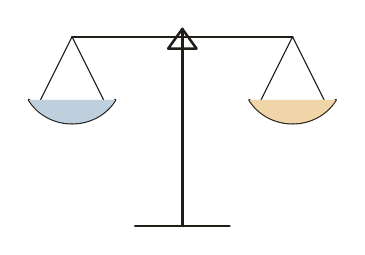
\begin{tikzpicture}[el]
  \draw[ink, line width=0.9pt] (0,-1.25)--(0,1.25);
  \draw[ink, line width=0.9pt] (-0.6,-1.25)--(0.6,-1.25);
  \draw[ink, line width=0.9pt] (0,1.25)--(-0.18,1.0)--(0.18,1.0)--cycle;
  \draw[ink, line width=0.9pt] (-1.4,1.15)--(1.4,1.15);
  \foreach \px/\pig in {-1.4/wwater, 1.4/wamber}{
     \draw[ink, line width=0.4pt] (\px,1.15)--(\px-0.4,0.35) (\px,1.15)--(\px+0.4,0.35);
     \draw[ink, line width=0.8pt] (\px-0.55,0.35) .. controls (\px-0.3,-0.05) and (\px+0.3,-0.05) .. (\px+0.55,0.35);
     \begin{scope}\clip (\px-0.55,0.35) .. controls (\px-0.3,-0.05) and (\px+0.3,-0.05) .. (\px+0.55,0.35) -- cycle;
        \fill[\pig!45] (\px-1,-0.3) rectangle (\px+1,0.5);\end{scope}}
\end{tikzpicture}}

\newcommand{\engCrystals}{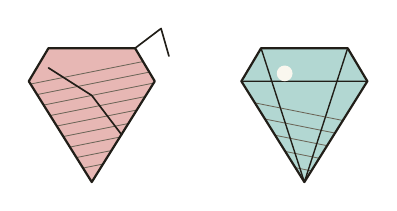
\begin{tikzpicture}[el]
  \def\lx{-1.35}
  \begin{scope}\clip (\lx-0.55,0.7)--(\lx+0.55,0.7)--(\lx+0.8,0.28)--(\lx,-1.0)--(\lx-0.8,0.28)--cycle;
     \fill[wred!40] (\lx-1,-1.1) rectangle (\lx+1,0.8);
     \foreach \hy in {-1,-0.85,...,0.3}{\draw[inkl,line width=0.3pt] (\lx-1,\hy)--(\lx+1,\hy+0.4);}\end{scope}
  \draw[ink, line width=0.8pt] (\lx-0.55,0.7)--(\lx+0.55,0.7)--(\lx+0.8,0.28)--(\lx,-1.0)--(\lx-0.8,0.28)--cycle;
  \draw[ink, line width=0.6pt] (\lx-0.55,0.45)--(\lx,0.1)--(\lx+0.38,-0.4);
  \draw[ink, line width=0.6pt] (\lx+0.55,0.7)--(\lx+0.88,0.95)--(\lx+0.98,0.6);
  \def\rx{1.35}
  \begin{scope}\clip (\rx-0.55,0.7)--(\rx+0.55,0.7)--(\rx+0.8,0.28)--(\rx,-1.0)--(\rx-0.8,0.28)--cycle;
     \fill[wteal!40] (\rx-1,-1.1) rectangle (\rx+1,0.8);
     \foreach \hy in {-1,-0.82,...,0.2}{\draw[inkl,line width=0.3pt] (\rx-1,\hy)--(\rx+1,\hy-0.4);}\end{scope}
  \draw[ink, line width=0.8pt] (\rx-0.55,0.7)--(\rx+0.55,0.7)--(\rx+0.8,0.28)--(\rx,-1.0)--(\rx-0.8,0.28)--cycle;
  \draw[ink, line width=0.5pt] (\rx-0.55,0.7)--(\rx,-1.0) (\rx+0.55,0.7)--(\rx,-1.0) (\rx-0.8,0.28)--(\rx+0.8,0.28);
  \fill[paper] (\rx-0.25,0.38) circle (0.1);
\end{tikzpicture}}

\newcommand{\engDials}{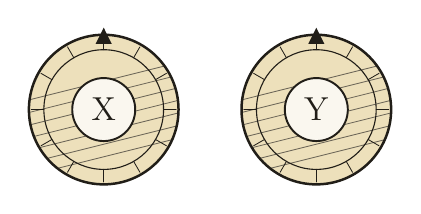
\begin{tikzpicture}[el]
  \foreach \x/\ch in {-1.35/X, 1.35/Y}{
     \begin{scope}\clip (\x,0) circle (0.95);\fill[wgold!35] (\x-1,-1) rectangle (\x+1,1);
        \foreach \hy in {-0.9,-0.74,...,0.2}{\draw[inkl,line width=0.3pt] (\x-1.2,\hy)--(\x+1.2,\hy+0.6);}\end{scope}
     \draw[ink,line width=0.9pt] (\x,0) circle (0.95);
     \draw[ink,line width=0.4pt] (\x,0) circle (0.76);
     \foreach \t in {0,30,...,330}{\draw[ink,line width=0.3pt] ($(\x,0)+(\t:0.76)$)--($(\x,0)+(\t:0.92)$);}
     \fill[ink] ($(\x,0)+(90:1.04)$)--($(\x,0)+(83:0.84)$)--($(\x,0)+(97:0.84)$)--cycle;
     \fill[paper] (\x,0) circle (0.4);\draw[ink,line width=0.7pt] (\x,0) circle (0.4);
     \node[ink,font=\large] at (\x,0) {\ch};}
\end{tikzpicture}}

\newcommand{\engGraph}{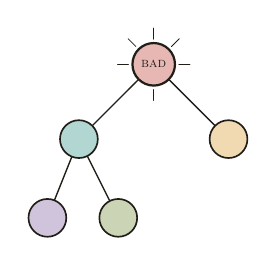
\begin{tikzpicture}[el]
  \coordinate (a) at (0,1.1);\coordinate (b) at (-0.95,0.15);\coordinate (c) at (0.95,0.15);
  \coordinate (d) at (-1.35,-0.85);\coordinate (e) at (-0.45,-0.85);
  \draw[ink,line width=0.5pt] (a)--(b) (a)--(c) (b)--(d) (b)--(e);
  \foreach \a in {0,45,...,315}{\draw[ink,line width=0.3pt] ($(a)+(\a:0.32)$)--($(a)+(\a:0.46)$);}
  \fill[wred!40] (a) circle (0.27);\draw[ink,line width=0.8pt] (a) circle (0.27);
  \node[ink,font=\tiny\scshape] at (a) {bad};
  \foreach \n/\pig in {b/wteal,c/wamber,d/wviolet,e/wgreen}{
     \fill[\pig!40] (\n) circle (0.24);\draw[ink,line width=0.6pt] (\n) circle (0.24);}
\end{tikzpicture}}

\begin{document}

% =====================================================================
% TITLE
% =====================================================================
\begin{frame}[plain]
  \vfill
  \centering
  {\engMountains}\\[1.2em]
  {\scshape\fontsize{34}{38}\selectfont Rotor in Rust}\\[0.5em]
  {\color{inkl}\rule{7cm}{0.4pt}}\\[0.7em]
  {\large Fast RISC-V machine-model generation, symbolic console\\
   arguments, and differential validation}\\[1.4em]
  {Jasmin Begi\'c \quad$\cdot$\quad Daniel Wassie}\\[0.3em]
  {\small\color{inkl} Advanced Systems Engineering, University of Salzburg
   \;\textbar\; supervised by Christoph Kirsch}\\[0.2em]
  {\small\color{inkl} June 2026}
  \vfill
\end{frame}

% =====================================================================
% CONTRIBUTIONS
% =====================================================================
\begin{frame}{Contributions}
  \vskip0.4em
  \begin{enumerate}\setlength\itemsep{0.9em}
    \item[\textsc{i.}] A \key{modular Rust reimplementation} of rotor ---
      same machine model and 24 properties, \key{$\sim$1000$\times$} faster
      generation in \key{21$\times$} less memory.
    \item[\textsc{ii.}] \key{Symbolic console arguments} --- a new input
      surface (the original paper's own future work), built with the paper's
      own formal device.
    \item[\textsc{iii.}] A \key{differential-validation methodology} ---
      \key{36/36} paired solver verdicts, and a back-port of the optimisation
      to the reference C ($\sim$95$\times$, byte-identical).
  \end{enumerate}
  \vfill
  \begin{block}{The thesis in one line}
    The speed-up is a \emph{data structure}, not a language; and the hard part
    is \emph{proving the new tool still tells the truth}.
  \end{block}
\end{frame}

% =====================================================================
% PROBLEM
% =====================================================================
\begin{frame}{Testing Samples; Verification Proves}
  \begin{columns}[T]
    \column{0.62\textwidth}
    \begin{itemize}\setlength\itemsep{0.6em}
      \item Testing runs a program on \emph{chosen} inputs. Eight bytes of
        input already give \key{$2^{64}$} possibilities --- a crash can hide
        anywhere untested.
      \item \emph{Bounded model checking} asks a single question over
        \emph{all} inputs, to depth $k$: \emph{can a bad state be reached?}
      \item \key{SAT} $\Rightarrow$ a concrete witness input that triggers it.
      \item \key{UNSAT} $\Rightarrow$ a guarantee, to depth $k$.
    \end{itemize}
    \column{0.34\textwidth}
    \vspace{1.1em}\centering
    \engSun\\[0.8em]
    {\small\itshape one question, asked of every input}
  \end{columns}
\end{frame}

% =====================================================================
% PIPELINE
% =====================================================================
\begin{frame}{Background: the Verification Pipeline}
  \begin{itemize}\setlength\itemsep{0.4em}
    \item \key{rotor} (part of selfie) translates a \emph{compiled} RISC-V
      binary into a bit-precise \key{BTOR2} machine model --- what is verified
      is what runs.
    \item \key{btormc} (Boolector) bounded-model-checks the model;
      \key{catbtor} checks well-formedness.
  \end{itemize}
  \vskip0.6em
  \begin{center}
  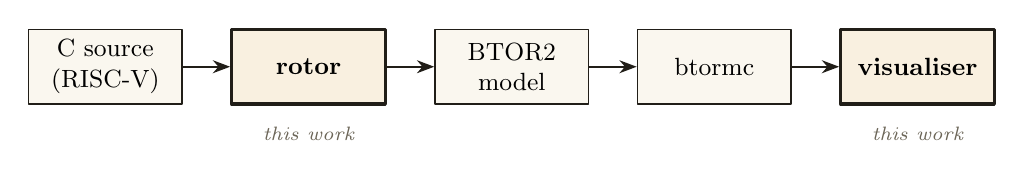
\begin{tikzpicture}[el, node distance=6mm,
     box/.style={draw=ink, line width=0.6pt, minimum width=1.95cm,
        minimum height=0.95cm, align=center, fill=paper, font=\small},
     ours/.style={box, line width=1.2pt, fill=wamber!16},
     ar/.style={-{Stealth[length=2.2mm]}, ink, line width=0.6pt}]
     \node[box] (a) {C source\\(RISC-V)};
     \node[ours, right=of a] (b) {\textbf{rotor}};
     \node[box, right=of b] (c) {BTOR2\\model};
     \node[box, right=of c] (d) {btormc};
     \node[ours, right=of d] (e) {\textbf{visualiser}};
     \draw[ar] (a)--(b);\draw[ar] (b)--(c);\draw[ar] (c)--(d);\draw[ar] (d)--(e);
     \node[font=\scriptsize\itshape, inkl, below=1.5mm of b] {this work};
     \node[font=\scriptsize\itshape, inkl, below=1.5mm of e] {this work};
  \end{tikzpicture}
  \end{center}
  \vskip0.2em
  \centering{\small The two highlighted stages are this project; selfie and
  btormc are unchanged third-party tools.}
\end{frame}

% =====================================================================
% WHAT A MODEL IS
% =====================================================================
\begin{frame}{What a Model Contains}
  \begin{columns}[T]
    \column{0.62\textwidth}
    \begin{itemize}\setlength\itemsep{0.5em}
      \item \key{State}: program counter, 32 registers, memory arrays
        (code, data, heap, stack), kernel counters.
      \item \key{Transitions}: one function per state variable --- the
        semantics of every instruction in the binary.
      \item \key{24 bad-state properties}: the things that must never happen.
    \end{itemize}
    \vskip0.5em
    {\small Examples: division-by-zero, segmentation faults, illegal
     instruction, stack-pointer violations, \emph{bad-exit-code}. Emission
     \emph{order} matters --- btormc identifies properties by index.}
    \column{0.34\textwidth}
    \vspace{0.6em}\centering
    \engGear\\[0.7em]
    {\small\itshape state, rules, and 24 forbidden squares}
  \end{columns}
\end{frame}

% =====================================================================
% CONTRIBUTION I -- THE REWRITE
% =====================================================================
\begin{frame}{\textsc{i.}\; Rotor in Rust --- a Modular Reimplementation}
  \begin{columns}[T]
    \column{0.62\textwidth}
    \begin{itemize}\setlength\itemsep{0.5em}
      \item Original: one \key{$\sim$14{,}000-line} C* file, hundreds of
        file-level globals.
      \item Rewrite: a modular crate --- \key{btor2}, \key{riscv},
        \key{machine}, \key{model}.
      \item Every BTOR2 node is a typed \texttt{enum Op}, hash-consed at
        creation; an explicit four-phase pipeline, no globals.
      \item Re-derived from \texttt{rotor.c} to emit the \key{same 24
        properties} in the \key{same order}.
    \end{itemize}
    \column{0.34\textwidth}
    \vspace{0.4em}\centering
    \engChest\\[0.6em]
    {\small\itshape one monolith $\rightarrow$ four clean parts}
  \end{columns}
\end{frame}

% =====================================================================
% PERFORMANCE
% =====================================================================
\begin{frame}{Performance}
  \begin{columns}[T]
    \column{0.58\textwidth}
    Modeling selfie compiled to itself (\key{43{,}406} RISC-U instructions):
    \vskip0.7em
    \begin{tabular}{l r r}
      \toprule
       & reference C & Rust\\
      \midrule
      Generation time & 139 s & \key{$<$0.1 s}\\
      Peak memory & 428 MB & \key{20 MB}\\
      \bottomrule
    \end{tabular}
    \vskip0.8em
    \begin{itemize}\setlength\itemsep{0.4em}
      \item $\sim$\key{1000$\times$} faster, \key{21$\times$} less memory.
      \item Measured fairly: both consume the \emph{same} pre-compiled
        binary, so compilation is excluded on both sides.
    \end{itemize}
    \column{0.38\textwidth}
    \vspace{1.0em}\centering
    \engHourglass\\[0.7em]
    {\small\itshape 139 seconds $\rightarrow$ a tenth of one}
  \end{columns}
\end{frame}

% =====================================================================
% THE COUNTING
% =====================================================================
\begin{frame}{The Cause: Counting the Hot Operation}
  Both tools repeat one question millions of times: \emph{``is this
  subexpression already built?''} We instrumented it.
  \vskip0.7em
  \begin{center}
  \begin{tabular}{l r r}
    \toprule
     & C rotor & Rust rotor\\
    \midrule
    Node creations & 3{,}171{,}632 & 159{,}018\\
    Dedup comparisons & \key{11{,}695{,}232{,}963} & \key{159{,}018}\\
    Output lines & 138{,}820 & 110{,}904\\
    \bottomrule
  \end{tabular}
  \end{center}
  \vskip0.6em
  \begin{itemize}\setlength\itemsep{0.3em}
    \item The C rotor answers by \key{walking a linked list} ($O(N)$ per node,
      $O(N^2)$ total); the Rust rotor by \key{one hash probe} ($O(1)$).
    \item Self-check: \emph{creations $-$ reuses $=$ each tool's own reported
      line count, to the integer.}
  \end{itemize}
\end{frame}

% =====================================================================
% THREE ROTORS
% =====================================================================
\begin{frame}{The Speed-up Is the Data Structure}
  Three rotors, one model --- proven by porting the change \emph{into the
  reference C itself}:
  \vskip0.6em
  \begin{center}
  \begin{tabular}{l r r r}
    \toprule
     & Original C & C + hash-consing & Rust\\
    \midrule
    Time & 139 s & 1.5 s & 0.1 s\\
    Memory & 428 MB & 485 MB & 20 MB\\
    Lines built & 3.17 M & 3.17 M & 159 k\\
    Output & \emph{baseline} & \key{byte-identical} & \emph{equivalent}\\
    Speed-up & 1$\times$ & $\sim$\key{95$\times$} & $\sim$\key{1000$\times$}\\
    \bottomrule
  \end{tabular}
  \end{center}
  \vskip0.5em
  \centering{\small The hashed C is byte-for-byte identical to the baseline
  and passes the same 36/36 check --- the cause was never the language.}
\end{frame}

% =====================================================================
% DEDUP COSMETIC
% =====================================================================
\begin{frame}{Deduplication Affects Size, Never Meaning}
  \begin{columns}[T]
    \column{0.62\textwidth}
    A supervisor's experiment --- disable line-reuse in both:
    \vskip0.5em
    \begin{itemize}\setlength\itemsep{0.5em}
      \item The reference C \key{crashes} (an internal sort-pointer
        invariant breaks) --- reuse there is \emph{load-bearing}, not just an
        optimisation.
      \item Rust runs unchanged: the model grows \key{1.43$\times$}, stays
        well-formed, and yields the \key{identical} solver verdict.
    \end{itemize}
    \vskip0.4em
    \textbf{Conclusion:} deduplication is cosmetic; meaning is preserved.
    \column{0.34\textwidth}
    \vspace{1.0em}\centering
    \engCrystals\\[0.7em]
    {\small\itshape C shatters; Rust holds}
  \end{columns}
\end{frame}

% =====================================================================
% CONTRIBUTION II -- SYMBOLIC ARGV
% =====================================================================
\begin{frame}{\textsc{ii.}\; Symbolic Console Arguments}
  \begin{columns}[T]
    \column{0.62\textwidth}
    \begin{itemize}\setlength\itemsep{0.5em}
      \item The original models stdin only; \key{argv was frozen} --- a whole
        class of bugs was structurally unreachable.
      \item We leave argument \emph{content} bytes as \key{uninitialized
        BTOR2 states} (the paper's own device for input); \texttt{argc},
        pointers and terminators stay concrete.
      \item Listed as \emph{future work} in the rotor paper.
      \item Verified: a program crashing only when \key{arg1='X'} \emph{and}
        \key{arg2='Y'} --- solved in seconds; five argv-only traps, all
        cracked.
    \end{itemize}
    \column{0.34\textwidth}
    \vspace{1.4em}\centering
    \engDials\\[0.7em]
    {\small\itshape the secret, found by reason}
  \end{columns}
\end{frame}

% =====================================================================
% CONTRIBUTION III -- VALIDATION METHOD
% =====================================================================
\begin{frame}{\textsc{iii.}\; Differential Validation --- the Criterion}
  \begin{columns}[T]
    \column{0.62\textwidth}
    Textual comparison is meaningless; formal equivalence is undecidable.
    Our checkable standard:
    \vskip0.4em
    \begin{block}{}
      For the same binary and parameters, both models must make the
      \key{same property index} satisfiable at the \key{same minimal bound
      $k$} --- or both stay UNSAT to the limit.
    \end{block}
    \vskip0.3em
    \begin{itemize}\setlength\itemsep{0.35em}
      \item $k$ is a \emph{fingerprint} of the whole run; one wrong
        instruction shifts it.
      \item Setup: 18 selfie benchmarks $\times$ 2 configurations; catbtor +
        btormc to $k=1500$.
    \end{itemize}
    \column{0.34\textwidth}
    \vspace{1.3em}\centering
    \engBalance\\[0.7em]
    {\small\itshape the solver as impartial referee}
  \end{columns}
\end{frame}

% =====================================================================
% VALIDATION RESULTS
% =====================================================================
\begin{frame}{Differential Validation --- Results}
  \begin{itemize}\setlength\itemsep{0.5em}
    \item \key{36/36} paired verdicts across two configurations --- zero
      divergences.
    \item Representative bounds: division-by-zero \key{@\,76}, load-seg-fault
      \key{@\,66}, bad-exit-code \key{@\,91--152}; one benchmark flips
      SAT/UNSAT under a parameter change --- and \emph{both rotors flip
      identically}.
    \item The criterion caught \emph{every} modeling defect during
      development --- and once caught an OOM artifact in our \emph{own}
      harness (one row disagreed with the other seventeen).
  \end{itemize}
  \vskip0.4em
  \begin{block}{What we do not claim}
    Not a formal proof of generator equivalence (undecidable). The evidence
    is bounded: 18 programs, depth 1500, two settings --- but it is
    falsifiable, and it \emph{was} falsified until it was not.
  \end{block}
\end{frame}

% =====================================================================
% VISUALIZER
% =====================================================================
\begin{frame}{Making Witnesses Legible}
  \begin{columns}[T]
    \column{0.62\textwidth}
    \begin{itemize}\setlength\itemsep{0.5em}
      \item btormc's witness is \key{thousands of lines of binary} keyed to
        internal node numbers --- sound, complete, and humanly opaque.
      \item A browser tool renders the model as an \key{interactive graph}
        and replays the witness on top; the bad state is highlighted at the
        violating step.
      \item Cone-of-influence views, collapsing, search, PNG/SVG export, 12
        preloaded examples.
      \item Online, no install: \texttt{jaspek.github.io/rotor-rust}.
    \end{itemize}
    \column{0.34\textwidth}
    \vspace{0.9em}\centering
    \engGraph\\[0.7em]
    {\small\itshape a wall of binary, made a picture}
  \end{columns}
\end{frame}

% =====================================================================
% CONCLUSIONS
% =====================================================================
\begin{frame}{Conclusions}
  \begin{itemize}\setlength\itemsep{0.35em}
    \item \key{Rotor in Rust} --- modular, $\sim$1000$\times$ faster,
      21$\times$ less memory; same 24 checks, solver-verified per benchmark.
    \item \key{Symbolic console arguments} --- the paper's future work; five
      argv-only bugs found by reason.
    \item \key{Differential validation} --- 36/36, plus a $\sim$95$\times$
      byte-identical C back-port: the cause is the data structure.
    \item A \key{witness visualizer} --- the answer made readable.
  \end{itemize}
  \vskip0.35em
  \begin{block}{The lesson}
    Not writing the code --- but \emph{proving the new one still tells the
    truth.}
  \end{block}
  \vskip0.25em
  {\footnotesize\color{inkl} Future work: symbolic argc / env / files; gcc
  binaries; semantic deduplication.}
\end{frame}

% =====================================================================
% CLOSE
% =====================================================================
\begin{frame}[plain]
  \vfill\centering
  {\engMountains}\\[1.2em]
  {\scshape\fontsize{26}{30}\selectfont Thank you}\\[0.6em]
  {\color{inkl}\rule{6cm}{0.4pt}}\\[0.8em]
  {\small\color{inkl} github.com/jaspek/rotor-rust \;\textbar\;
   rotor-c-hashcons \;\textbar\; jaspek.github.io/rotor-rust}
  \vfill
\end{frame}

\end{document}
